%%%%%%%%%%%%%%%%%%%%%%%%%%%%%%%%%%%%%%%%%%%%%%%%%%%%%%%%%%%%%%%%%%%%%
%
% Axel Fahy & Höhn Rudolf
% Automn Semester MSE
% IV
%
%%%%%%%%%%%%%%%%%%%%%%%%%%%%%%%%%%%%%%%%%%%%%%%%%%%%%%%%%%%%%%%%%%%%%%

\documentclass[11pt]{report}
%\documentclass[twoside, openright]{report}                           % To print on twoside
\usepackage[a4paper]{geometry}
\usepackage[T1]{fontenc}
\usepackage[utf8]{inputenc}
\usepackage[myheadings]{fullpage}
\usepackage{lastpage}
\usepackage{graphicx, wrapfig, subcaption, setspace, booktabs}
\usepackage[font=small, labelfont=bf]{caption}
\usepackage{fourier}
\usepackage[protrusion=true, expansion=true]{microtype}
\usepackage{amsmath}
\usepackage{sectsty}
\usepackage{hyperref}                                                 % Links are clickable
\usepackage{url, lipsum}
\usepackage{parskip}                                                  % Remove identation
\usepackage{emptypage}                                                % Do not print page number on empty pages
\usepackage{float}
\usepackage[absolute]{textpos}
\usepackage{fancyvrb}
\usepackage[export]{adjustbox}

\bibliographystyle{unsrt}

%-------------------------------------------------------------------------------
% MARGIN SETTINGS
%-------------------------------------------------------------------------------
\geometry{
	paper=a4paper, % Change to letterpaper for US letter
	inner=2.5cm, % Inner margin
	outer=3.5cm, % Outer margin
	bindingoffset=1.5cm, % Binding offset
	%top=1.5cm, % Top margin
	%bottom=1.5cm, % Bottom margin
	%showframe,% show how the type block is set on the page
}

%-------------------------------------------------------------------------------
% LIST DIRECTORIES
%-------------------------------------------------------------------------------
\usepackage[dvipsnames]{xcolor}                                       % Color names
\usepackage{dirtree}                                                  % List directories
\renewcommand*\DTstylecomment{\rmfamily\color{Gray}\textsc}           % Color of comments
\renewcommand*\DTstyle{\ttfamily\textcolor{OliveGreen}}               % Color of stucture
\setlength{\DTbaselineskip}{12pt}                                     % Skip between lines
\DTsetlength{1em}{1em}{0.1em}{1pt}{2pt}                               % Lines format

%-------------------------------------------------------------------------------
% CODE FORMAT
%-------------------------------------------------------------------------------
\usepackage{listings}                                                 % Code listings
\usepackage{listingsutf8}
\lstset{inputencoding=utf8/latin1}
\usepackage[dvipsnames]{xcolor}
\definecolor{mygreen}{rgb}{0,0.6,0}
\definecolor{mygray}{rgb}{0.5,0.5,0.5}
\definecolor{mymauve}{rgb}{0.58,0,0.82}
\definecolor{bggray}{rgb}{0.95, 0.95, 0.95}
\lstset{ %
    backgroundcolor=\color{bggray},   % choose the background color; you must add \usepackage{color} or \usepackage{xcolor}
    basicstyle=\footnotesize,        % the size of the fonts that are used for the code
    breakatwhitespace=false,         % sets if automatic breaks should only happen at whitespace
    breaklines=true,                 % sets automatic line breaking
    captionpos=b,                    % sets the caption-position to bottom
    commentstyle=\color{mygreen},    % comment style
    deletekeywords={}            % if you want to delete keywords from the given language
    escapeinside={\%*}{*},          % if you want to add LaTeX within your code
    extendedchars=true,              % lets you use non-ASCII characters; for 8-bits encodings only, does not work with UTF-8
    frame=single,                    % adds a frame around the code
    frameround=tttt                  % tttt for having the corner round.
    keepspaces=true,                 % keeps spaces in text, useful for keeping indentation of code (possibly needs columns=flexible)
    keywordstyle=\color{blue},       % keyword style
    language=html,                 % the language of the code
    morekeywords={*},            % if you want to add more keywords to the set
    numbers=none,                    % where to put the line-numbers; possible values are (none, left, right)
    numbersep=5pt,                   % how far the line-numbers are from the code
    numberstyle=\tiny\color{mygray}, % the style that is used for the line-numbers
    rulecolor=\color{black},         % if not set, the frame-color may be changed on line-breaks within not-black text (e.g. comments (green here))
    showspaces=false,                % show spaces everywhere adding particular underscores; it overrides 'showstringspaces'
    showstringspaces=false,          % underline spaces within strings only
    showtabs=false,                  % show tabs within strings adding particular underscores
    stepnumber=1,                    % the step between two line-numbers. If it's 1, each line will be numbered
    stringstyle=\color{mymauve},     % string literal style
    tabsize=2,                       % sets default tabsize to 2 spaces
    title=\lstname}                 % show the filename of files included with \lstinputlisting; also try caption instead of title

%-------------------------------------------------------------------------------
% COMMAND LINE FORMAT
%-------------------------------------------------------------------------------
\lstdefinestyle{CommandLineStyle}{
    backgroundcolor=\color{black},
    basicstyle=\color{white}\footnotesize\ttfamily,
    breakatwhitespace=false,
    breaklines=true,
    captionpos=b,
    deletekeywords={},
    escapeinside={\%*}{*},
    extendedchars=true,
    frame=none,
    keepspaces=true,
    numbers=none,
    rulecolor=\color{black},
    showspaces=false,
    showstringspaces=false,
    showtabs=false,
    tabsize=2,
    deletekeywords={default}}
%-------------------------------------------------------------------------------
% INLINE FORMAT
%-------------------------------------------------------------------------------
\lstdefinestyle{InlineStyle}{
    basicstyle=\footnotesize,
    breakatwhitespace=false,
    breaklines=true,
    captionpos=b,
    deletekeywords={},
    escapeinside={\%*}{*},
    extendedchars=true,
    frame=none,
    keepspaces=true,
    keywordstyle=\color{blue},
    language=java,
    morekeywords={*},
    showspaces=false,
    showstringspaces=false,
    showtabs=false,
    tabsize=2}


\newcommand{\HRule}[1]{\rule{\linewidth}{#1}}
\onehalfspacing{}
\setcounter{tocdepth}{5}
\setcounter{secnumdepth}{5}

\usepackage{titlesec}
%\titleformat{\chapter}{}{}{0em}{\bf\LARGE}      % Remove the 'Chapter' before each chapter
%\titleformat{\chapter}{\normalfont\huge}{\thechapter.}{20pt}{\huge\it}
\titleformat{\chapter}{\normalfont\huge}{\thechapter.}{20pt}{\huge}
\titlespacing*{\chapter}{0pt}{-50pt}{30pt}      % Change 'before' spacing (default is 50pt) and 'after' spacing (default is 40pt)
%\makeatletter
%\renewcommand{\@makechapterhead}[1]{%
%\vspace*{0 pt}%
%\bfseries\Huge\thechapter.\ #1
%\par\nobreak\vspace{40 pt}}}
%\makeatother

\usepackage{pdfpages}                                                 % To include another pdf

%-------------------------------------------------------------------------------
% HYPERLINKS CONF
%-------------------------------------------------------------------------------
\hypersetup{colorlinks=true}

%-------------------------------------------------------------------------------
% HEADER & FOOTER
%-------------------------------------------------------------------------------
\usepackage{fancyhdr}
\pagestyle{fancy}
\fancyhf{}
\setlength\headheight{15pt}
\fancyhead[L]{\textsl{\leftmark}}
\fancyfoot[L]{\textsl{Axel} FAHY \& \textsl{Rudolf} HÖHN}
\fancyfoot[R]{\thepage}
\renewcommand{\footrulewidth}{0.4pt}    % Horizontale line for footer
% Redefine the plain page style
\fancypagestyle{plain}{
  \fancyhf{}
  \fancyfoot[R]{\thepage}
  \renewcommand{\headrulewidth}{0pt}    % Line at the header invisible
  \renewcommand{\footrulewidth}{0pt}    % Line at the footer visible
}

\begin{document}
%-------------------------------------------------------------------------------
% TITLE PAGE
%-------------------------------------------------------------------------------
\title{Stocks Trooper\\Information Visualization\\MSE}
\date{\today\\\href{https://github.com/rudy2707/Stockstrooper}{GitHub repository}}
\author{Axel Fahy \& Rudolf Höhn}
\maketitle

\tableofcontents

\pagestyle{fancy}     % Print page number again

%-------------------------------------------------------------------------------
% CHAPTER INTRODUCTION
%-------------------------------------------------------------------------------
\chapter{Introduction}
\label{chapter:introduction}
In this chapter, we define what is the aim of the project, the different features and mockups we are implementing and finally, the different technologies we are using.

%-------------------------------------------------------------------------------
%-------------------------------------------------------------------------------
\section{Aim of the project}
This projects aims to detect important events on stocks values and present them on a GUI.\@ An event is understood as a ''\textit{significant decrease or increase in a short amount of time}''. For each event, the application will suggest relevant articles to help the user have a better understanding.

%-------------------------------------------------------------------------------
%-------------------------------------------------------------------------------
\section{Features to implement}
These following features must appear in the application:
\begin{enumerate}
    \item Display the stocks values of a particular index between two dates
    \item Display on a timeline the events detected in the stocks values
    \item Display some news articles related to the event
\end{enumerate}

%-------------------------------------------------------------------------------
%-------------------------------------------------------------------------------
\section{Technologies used}
Python and AngularJS are the two main programming languagues we are using in this application. In addition to the language, we are using the following libraries:
\begin{itemize}
    \item flask
    \item pandas
    \item yahoo\_finance
\end{itemize}


%-------------------------------------------------------------------------------
% CHAPTER SPECIFICATIONS
%-------------------------------------------------------------------------------
\chapter{Specifications}
\label{chapter:specifications}
In this chapter, we describe precisely the IT related specifications (e.g. REST routes, data format, GUI).

%-------------------------------------------------------------------------------
%-------------------------------------------------------------------------------
\section{System architecture}
TODO graphical representation of the system

%-------------------------------------------------------------------------------
%-------------------------------------------------------------------------------
\section{Flow diagram}
The figure~\ref{fig:specs:flowdiagram} defines precisely how the user interacts with the application. It allows to have a clear representation of the system.

\begin{figure}[H]
    \centering
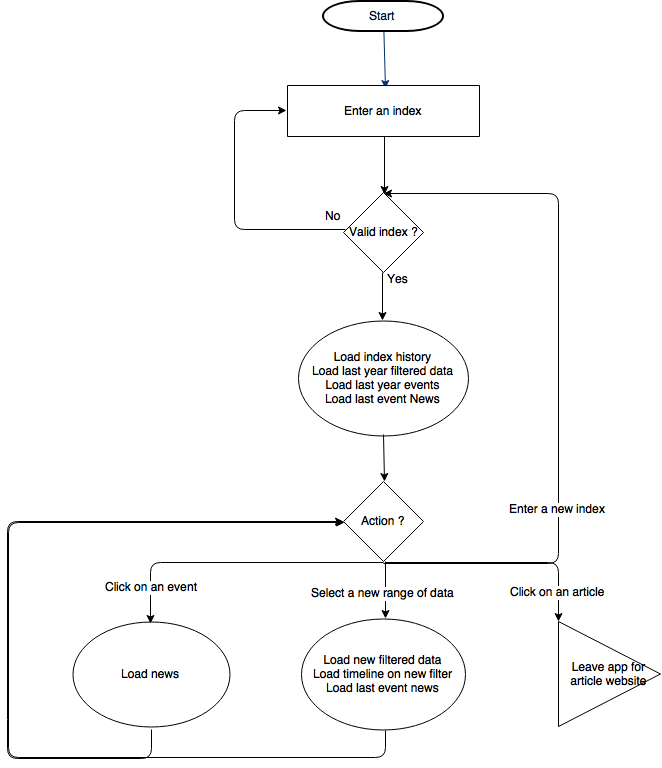
\includegraphics[scale=0.5]{Figures/workflow-stockstrooper.png}
\caption{Flow diagram of the user interaction}
\label{fig:specs:flowdiagram}
\end{figure}

%-------------------------------------------------------------------------------
%-------------------------------------------------------------------------------
\section{REST API}

%-------------------------------------------------------------------------------
\subsection{Routes and format}

\subsubsection*{GET events}
This route sends all events within a period for one index. Default is one year from present. With each event comes its trend. A positive event has a value of \textit{1} and a negative one a value of \textit{-1}.
\begin{verbatim}
/events/:index[/:datestart/:dateend]

[
    {
        "date": "20160502",
        "trends": -1
    },
    {
        "date": "20160716",
        "trends": -1
    },
    {
        "date": "20150123",
        "trends": 1
    }
]
\end{verbatim}

\subsubsection*{GET stocks}
This route sends all the stocks data for one index (market index).
\begin{verbatim}
/stocks/:index

[
      [
            345427200000000000,
            0.426842
      ],
      [
            345686400000000000,
            0.404572
      ],
      [
            345772800000000000,
            0.374879
      ]
]
\end{verbatim}

\subsubsection*{GET news}
This route sends all the news related to one index and one event.
\begin{verbatim}
/news/:index/:dateevent

[
    {
        "url": "http://www.nytimes.com/reuters/2016/01/08/business/
                08reuters-apple-stock-research.html",
        "headline": "Wall St. Bets on Apple Bounceback Despite
                     iPhone Shipment Worries",
        "date": "2016-01-08T09:36:56Z",
        "source": "Reuters"
    }
]
\end{verbatim}

\subsubsection*{GET index valid}
This route sends a boolean variable which indicates if the index is valid or not.
\begin{verbatim}
/index/:index/

{
    "valid": true
}
\end{verbatim}
%-------------------------------------------------------------------------------
\subsection{CORS}

The \textit{CORS} problems were handle with \textit{Flask}.

%-------------------------------------------------------------------------------
\subsection{Detection of events}

The events of a company are detected by searching the biggest changes of share value during a short period of time.

To do this, a threshold is calculated in order to define if the changes of share will be considered as an event.

\begin{lstlisting}[language=python, belowskip=-1.0 \baselineskip]
    threshold = (max(values) - min(values)) * 0.09
\end{lstlisting}

This allows to have a threshold that varies depending on the volatility of the actions. In order to avoid having a threshold to big, the $90\%$ of the calculated value is taken.

Afterwards, we take all the data and process them by samples of a specific size (default value is a size of 10 values). In this current sample, we will calculate the difference between the maximum and the minimal value. If this value exceeds the threshold, this sample will be considered as an event. The sample is composed of multiple dates, the middle date of the sample is chosen to represent the event.

Depending of the stock we are processing, we may have more or less events that we wanted. If we have found more events, we take the highest events and keep them. Events will be sorted by highest difference between max and min value in order to know which ones are the most important. However, if we have less events, the threshold is decrease by $0.05$ and we process all the samples all over again until we have enough events.








%-------------------------------------------------------------------------------
% CHAPTER IV
%-------------------------------------------------------------------------------
\chapter{Information Visualisation aspects}
\label{chapter:iv}
In this chapter, we describe all the choices and aspects of the application related to the purpose of the course which is the Information Visualisation. We also cover a part of User Experience.

%-------------------------------------------------------------------------------
%-------------------------------------------------------------------------------
\section{Target audience}
This app is provided to different financial actors, from analysts, to managers and even students. It helps the user to create a mental model bringing together what were the stocks values at some time and what appeared in the news around this event, which might lead to be an answer and to understand the evolution of the price.

%-------------------------------------------------------------------------------
%-------------------------------------------------------------------------------
\section{Data to visualize}
The first question to ask is what is the data we are using and what information we want to give to the user. As stated in section~\ref{sec:intro:features}, we want to give a clear picture of the different events that occured within a specific range of time (e.g. 1 year) by providing news related to the events.
For example, if the shared stock value of some company dropped on 3$^{\text{rd}}$ July 2015, the user might want to know what happened on this particular day. Thus, the app will retrieve the news that talk about the company around that day. Maybe that an article from \textit{Reuters} or \textit{Swissquote} will explain why the shared stock value lost 50 \$.

The data is numerical, quantitative and temporal (i.e. expressed with a time dimension). Defaults are set to present 1 year from the current day of stock values, 5 events occuring in this time frame, and the articles in a range of 2 months before and after the event.

In the next sections, we are describing more precisely the different information present on the app and how we decided to represent them.

%-------------------------------------------------------------------------------
\subsection{Stock values}
To represent the stock values we used a chart created with the Javascript library HighchartsJS, or more specifically, with HighstocksJS, a library using HighchartsJS. In the figure~\ref{fig:stockchart}, we see Facebook (FB) stock prices in a one year time range.
\begin{figure}
    \centering
    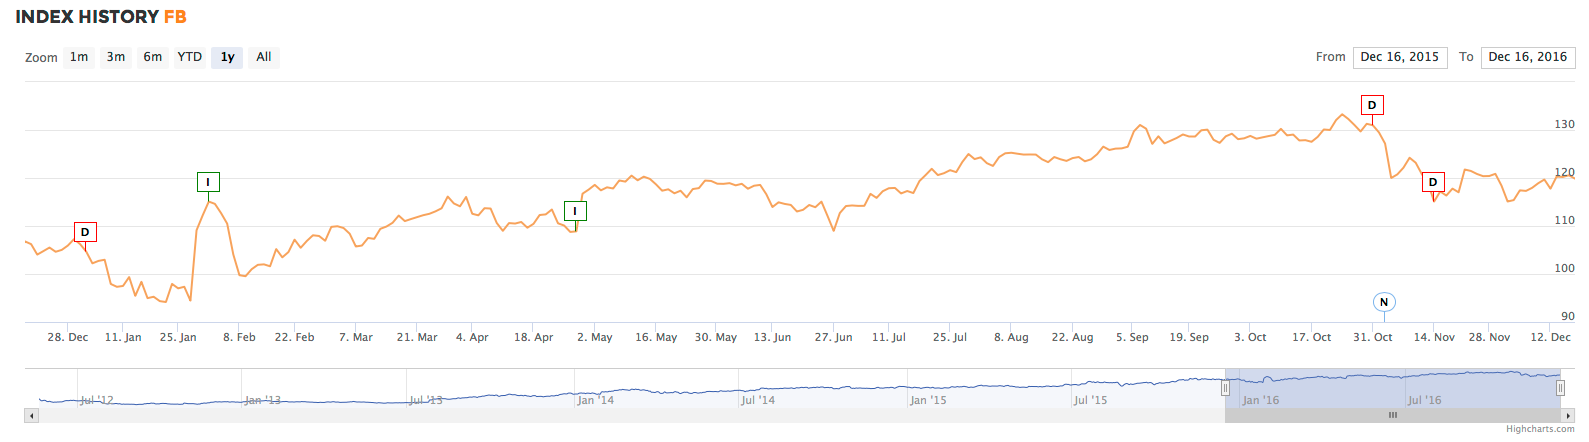
\includegraphics[scale=0.24]{Figures/stock-values.png}
    \caption{Example of visualisation of the Facebook (FB) stock price between the 16$^{\text{th}}$ December 2015 and 16$^{\text{th}}$ December 2016.}
    \label{fig:stockchart}
\end{figure}
There are two important visual enhancements to a simple line chart present in our chart. First, there are two visualization of the data itself, one big of current timeframe and a second one smaller below the big one representing briefly the whole data set. And secondly, the different events were added as flags on the line to let the user visualize at first sight when the events occured. The flags are here to amplify cognition.

In addition of the visual enhancements, there is also the possibility to interact directly with the chart and zoom to a particular range or to drag the mouse and know what we are pointing at.

As our target is financial actors, representing the line chart is what they are used to when they look at the evolution of the stock price. Thus, in order to be the least surprising to them, we decided to also use a line chart.

%-------------------------------------------------------------------------------
\subsection{Events}
Before getting at how we represented the events, let us define what an event is.
\begin{center}
    An event is understood as a ``\textit{significant decrease or increase in a short amount of time}''.
\end{center}
An event is linked to the information provided by the line chart. In order to keep this temporal dimension, we decided to represent the events on a non-scaled (i.e. the separation between the dates does not respect the actual time difference) timeline. The timeline is top-bottom, which means that the most recent event is at the top and the others follow in a reversed chronological order.

Besides the time information, we also represent the type of event. Is it an event due to a significant increase (i.e. positive event) or decrease (i.e. negative event)? To answer this question, let us consider the figure~\ref{fig:event-timeline}. An arrow facing up describes a positive event and, \textit{a contrario}, an arrow facing down describes a negative event. This information is amplified by the color. A green or red arrow is used for respectively a positive or a negative event.

The highlighted event helps the user to reminder what event is currently used to retrieve the news.

% TODO Correct the text on the figure

\begin{figure}
    \centering
    % 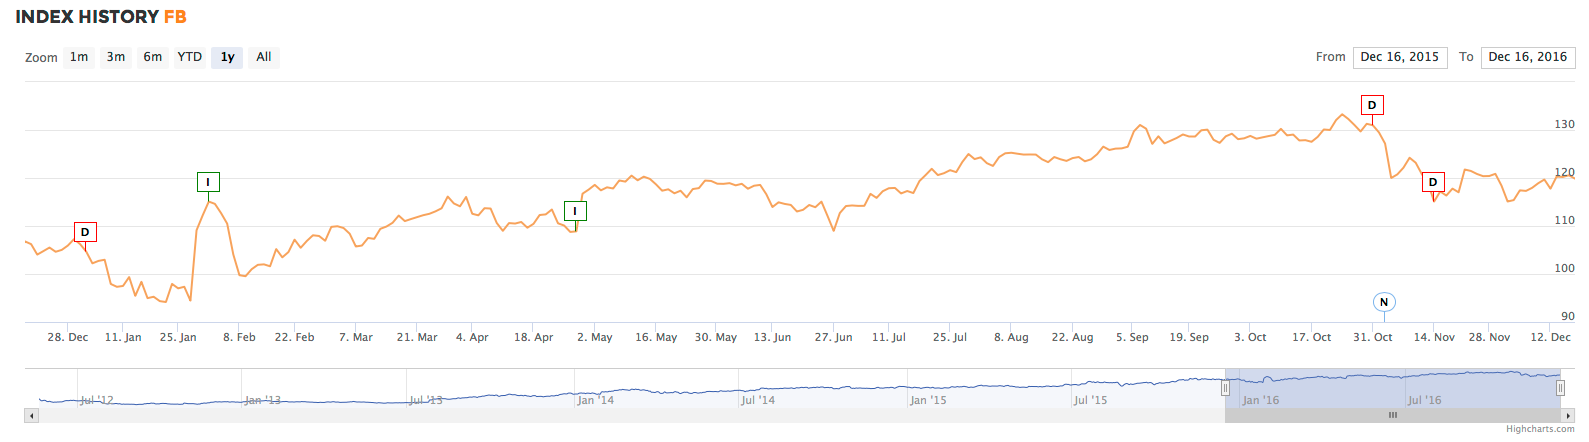
\includegraphics[scale=0.24]{Figures/stock-values.png}
    \textbf{Here add the screenshot of the timeline of events}
    \caption{Example of visualisation of the Facebook (FB) stock price events between the 16$^{\text{th}}$ December 2015 and 16$^{\text{th}}$ December 2016.}
    \label{fig:event-timeline}
\end{figure}

%-------------------------------------------------------------------------------
\subsection{News}
simple list with highlights

%-------------------------------------------------------------------------------
%-------------------------------------------------------------------------------
\section{One page design}
why one page design
why chart left + timeline right => eyes path

%-------------------------------------------------------------------------------
%-------------------------------------------------------------------------------
\section{The orange color}
As shown in the third lecture\footnote{InfoVisMSE\_03.pdf, p.13} of the course, a different color helps the perception as a \textit{preattentive processing}, for example to highlight information. In our case, what we are highlighting is the data that changes through the use of the application. Here is the list of orange representation on the application.
\begin{itemize}
    \item Line in the chart
    \item Current index
    \item Events range
    \item News relevant to an event
\end{itemize}
The purpose is to catch the eye when the user does not remember the context of what he is looking at and needs a refresh.

%-------------------------------------------------------------------------------
%-------------------------------------------------------------------------------
\section{User Experience}
one page design
loading spinkits
interactions: explore (stocks options value, news), reconfigure (events on timeline, events as flags on chart), abstract / elaborate (change date range), connect (select a range changes the events, select an event changes the news)
tasks: overview, zoom, detail on demand, history

%-------------------------------------------------------------------------------
%-------------------------------------------------------------------------------
\section{Easter egg}
This is a secret section. However, if you gently ask a Storm Trooper, he might reveal it.


%-------------------------------------------------------------------------------
% CHAPTER CONCLUSION
%-------------------------------------------------------------------------------
\chapter{Conclusion}
\label{chapter:conclusions}

%-------------------------------------------------------------------------------
%-------------------------------------------------------------------------------
\section{Project status}
The application is usable and respect the features described in th section \ref{sec:intro:features}. However, in software development context, some steps are missing, like the user testing. This is the first draft and it needs refinement.

In terms of performance, there is an open issue on Github that describes the problem.

%-------------------------------------------------------------------------------
%-------------------------------------------------------------------------------
\section{Future work}

\subsection{Improvement on the UX}
Here is a non-exaustive list of things that can be improved within the UX aspect.
\begin{itemize}
    \item \textbf{Override the defaults}: the default range of 1 year, the number of events, etc. Maybe we can integrate these customizations and preferences as a user profile.
    \item \textbf{News time range around the event}: on an event time range of 1 year, the list of news is filled with articles that might have been published $\pm$ 2 months around the event. This is a ratio of about $\frac{1}{6}$ of the event time range to retrieve the news. It might be relevant to remove this 2 months security, but instead to keep this ratio and always provide a $\frac{1}{6}$ ratio between the events and the news time range. For example, for an event time of 1 month, we could have articles of $\pm$ 5 days around the event.
    \item \textbf{History of use}: it might be interesting to have some sort of a list that contains all the requests made by the user. This way, he can go back to a previous state of the application and analyze the data as previously.
\end{itemize}

Although this list does not contain all the possible improvements on the UX, the best way to find other aspects to take into consideration is to do a real user testing with real end-users.

\subsection{Diversify the sources of the data}
Currently, the application only bases its news data on the \textit{New York Times API} and they suffer of a lack of articles. An improvement could be to integrate other APIs of news companies or press agencies to give to the user the best knowledge he deserves.


\appendix
%-------------------------------------------------------------------------------
% APPENDIX 1
%-------------------------------------------------------------------------------
\include{Appendices/Appendix1}

% \begin{table}
% \caption{Example of a Machine Learning algorithm prediction abilities}
% \label{tab:ml-example}
% \centering
% \begin{tabular}{l l l | l}
% \toprule
% \tabhead{Color} & \tabhead{Diameter $[cm]$} & \tabhead{Fruit} & \tabhead{Chances of good prediction}\\
% \midrule
% Red & 5 & Apple & Good\\
% Orange & 5 & Orange & Good\\
% Orange & 8 & Apple & Very bad\\
% Yellow & 10 & Orange & Bad\\
% \bottomrule\\
% \end{tabular}
% \end{table}

\end{document}
